% Why it is not straightforward to evaluate LLM's output for this. Because KBQA answers are list of entities, but output is freetext. Propose to use an independent LLM (Gemini) to assist in evaluating. 

\begin{listing}[t]
\begin{minted}[breaklines=true,fontsize=\small]{text}
You are evaluating a question answering task. The ground-truth answer is a list of answer-items. 
First, extract the answer-items from the generated answer. 
Then, map each generated answer-item to the ground-truth answer-item if possible. If no matching, use an empty list.
Output using the following format. {"predicted_answer": [list of answer-items extracted from the generated answer], "mappings": {"predicted_answer_1": [matched groundtruth answers], "predicted_answer_2": []}}

Question: <KBQA Question>
Ground-truth answer: <KBQA Ground-truth Answer>
Generated answer: <LLM-generated Answer>
\end{minted}
\caption{Prompt template for KBQA evaluation using Gemini Pro. The actual content will be filled in the placeholders of \textit{Question}, \textit{Ground-truth answer}, and \textit{Generated answer}. }
\label{list:gemini_prompt}
\end{listing}

\begin{figure}
    \centering
    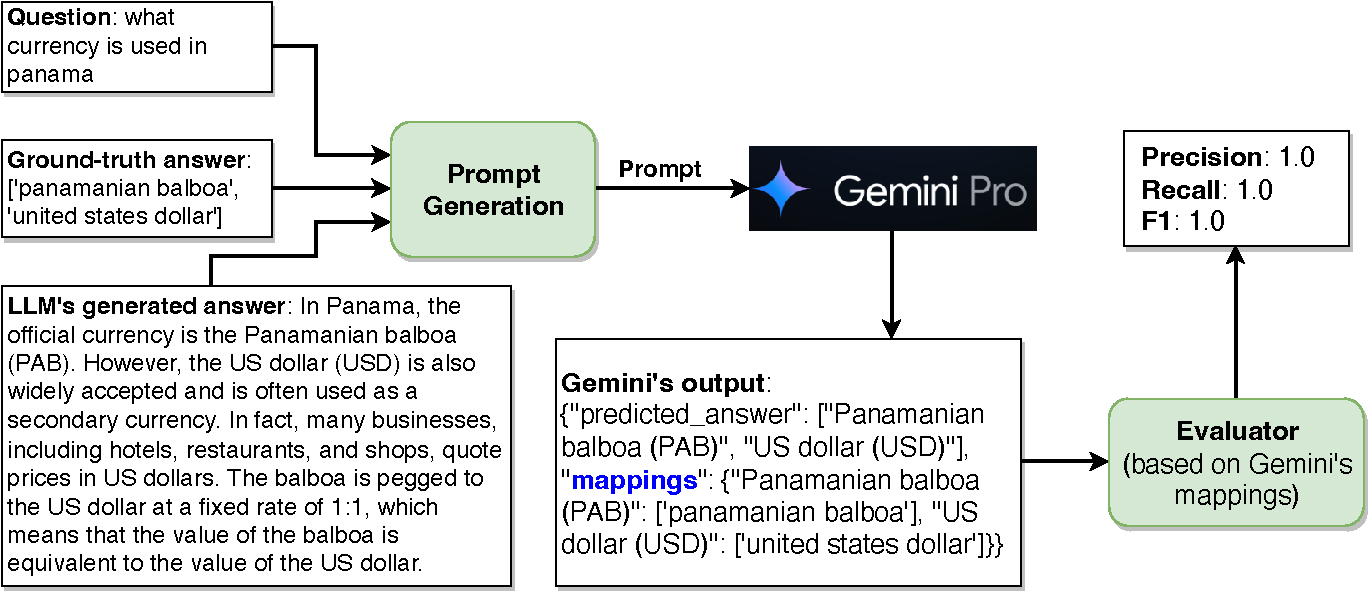
\includegraphics[width=.5\textwidth]{image/gemini_eval.pdf}
    \caption{LLM-based KBQA evaluation workflow using prompts for precision, recall, and F1 scores with Gemini-1.0-Pro as evaluator.}
    %\caption{LLM-based KBQA Evaluation Workflow. Given the input of \textit{question}, \textit{ground-truth answer}, and \textit{LLM's generated answer}, we create a prompt to extract answer-items and map them to ground-truth answer-items. Then, we calculate the precision, recall, and F1 based on the mappings of generated and ground-truth answer-items. We use Gemini-1.0-Pro for this evaluation task.} %The generated answer is taken from Llama 3-8B. }
    \label{fig:gemini_eval}
\end{figure}

% In KBQA task, the most common type of answer is a list of entities from the KG. For example, the answer to the question ``What language is spoken in Switzerland?'' is ``[Italian language, German language, French, Romansh language]''. While we can request LLMs to generate answers in the format of a list of entities, not all LLMs consistently follow this output format request. Therefore, it is crucial to process the answers returned by LLMs to extract the entity list for evaluation. One solution is to use Named Entity Recognition (NER); however, answers can contain other types of information besides named entities. Additionally, the wording used in answers might differ from the KG's entities even though they refer to the same entity, such as ``United States Dollar'' versus ``US dollar (USD)''.

% To resolve this problem, we propose an LLM-based evaluation method where an LLM is requested to extract answer-items (entities) from the generated answer and map them to the ground-truth answer-items. Figure \ref{fig:gemini_eval} shows the LLM-based KBQA evaluation workflow with an actual example using an answer generated from Llama 3-8B. We first construct a prompt using our pre-defined prompt template, shown in Listing \ref{list:gemini_prompt}. The prompt contains the input question, ground-truth answer, LLM's generated answer, and a request to extract answer-items and map them to the ground-truth answer-items. As shown in Figure \ref{fig:gemini_eval}, Gemini outputs a list of \textit{predicted answers} and a \textit{mapping} which maps each item in the predicted answers with those in ground-truth answers. Noted that one predicted answer-item can be mapped to more than one ground-truth answer-item or none (i.e., wrong answer). 

In the KBQA task, answers are typically lists of entities from the KG. For instance, the answer to ``What language is spoken in Switzerland?'' is ``[Italian, German, French, Romansh]''. While LLMs can be asked to generate entity lists, they do not always follow this format. Therefore, processing LLM-generated answers to extract entity lists for evaluation is crucial. Using Named Entity Recognition (NER) alone is not sufficient because answers may include non-entity information and differing entity wordings, e.g., ``United States Dollar'' versus ``US dollar (USD)''.
To address this, we propose an LLM-based evaluation method where an LLM extracts and maps answer-items (entities) from the generated answer to the ground-truth entities. Figure \ref{fig:gemini_eval} illustrates this workflow with an example generated by Llama-3-8B. We construct a prompt using a predefined template (Listing \ref{list:gemini_prompt}), including the question, ground-truth answer, LLM-generated answer, and a request for entity extraction and mapping. As shown in the figure, Gemini outputs a list of \textit{predicted answers} and a \textit{mapping} of predicted answers to ground-truth answers. A predicted answer can map to multiple ground-truth items or none (i.e., incorrect answer).

The mapping is then used to compute evaluation metrics including Precision, Recall, and F1. The details are as follows. 
Given a question, we denote the ground-truth answer as $A=[A_1, A_2, \cdots, A_n]$ and the list of predicted answer-items as $\hat{A}=[\hat{A}_1, \hat{A}_2,\cdots, \hat{A}_m]$. The mapping is denoted as $M=\{\hat{A}_1: M_1, \hat{A}_2: M_2, \cdots, \hat{A}_m: M_m\}$ where $M_i$ is a list of ground-truth answer-items matched with the corresponding predicted answer-item, i.e., $M_i \subseteq A$ ($i=1, \cdots, m$) and $M_i$ is empty when the predicted answer-item is wrong. A predicted answer-item is called \textit{correct} if it matches with at least one of the ground-truth answer-items.
We define $c_G=|\text{set}(M_1\cup M2 \cup \cdots \cup M_m)|$ as the number unique ground-truth answer-items that matched with at least one predicted answer-item and $c_P$ as the number of correct predicted answer-items. The final number of correct answers is chosen as the smallest number between $c_G$ and $c_P$. 
% :
% \begin{align}
%     c = \left\{\begin{matrix}
% c_G & \text{if } c_G < c_P\\ 
% c_P & \text{otherwise} 
% \end{matrix}\right.
% \end{align}
This is to deal with the cases where different predicted answer-items carry the same meaning (mapped to the same ground-truth answer-item). The precision and recall are then computed as $\frac{c}{|\hat{A}|}$ and $\frac{c}{|A|}$, respectively. 
% follows: 
% \begin{align}
%     \text{precision} = \frac{c}{|\hat{A}|}
% \end{align}
% \begin{align}
%     \text{recall} = \frac{c}{|A|}
% \end{align}
F1 score is computed as the harmonic mean of precision and recall. 
We chose \gemini for this evaluation task because of its strong natural language processing capabilities and its availability during our experiments.